\section{TDM测试环境说明}
\subsection{关于测试环境相关文件}
\begin{itemize}
\item 服务器SDK工程,SDK工程路径:
\begin{messagebox}
/230common/mozhiye/BR30/br30_tdm_test_env_20200819
\end{messagebox}
\item 下载目录:
\begin{messagebox}
BR30_tdm_test_download.zip
\end{messagebox}
\item 骨传导传感器\href{https://www.st.com/resource/en/datasheet/lis25ba.pdf}{LIS25BA规格书};
\end{itemize}

\subsection{关于测试环境相关驱动文件组成}
\begin{itemize}
\item 传感器驱动文件:SDK/apps/common/device/gSensor/lis25ba.c
\item TDM接口驱动文件:SDK/lib/media/media\_new/cpu/br30/audio\_link.c
\item 修改数据接收方式头文件:SDK/include\_lib/driver/cpu/br30/asm/tdm\_test.h
\end{itemize}

\subsection{关于SDK修改}
由于ALINK接收数据位宽的限制(最大24bit),因此同一时刻只能接收传感器输出的X,Y,Z轴数据的其中两个轴数据,修改接收不同轴数据,需修改tdm\_test.h文件,选择需要接收的数据;
\begin{myccode}[caption={tdm\_test.h}]
#ifndef _TDM_TEST_H_
#define _TDM_TEST_H_

//===========================================//
//              接收TDM数据选择:二选一      //
//===========================================//
#define TDM_GET_X_Y_AXIS_DATA 		//选择接收X, Y数据
//#define TDM_GET_X_Z_AXIS_DATA     //选择接收X, Z数据

#define TDM_PUT_RAW_DATA

#endif /* #ifndef _TDM_TEST_H_ */
\end{myccode}

修改该文件后需要make工程并更新固件到小机,重新上电接收数据;


\subsection{关于串口数据接收工具使用}
\emphasizebox{SerialReadData.exe}工具可以将接收到的数据以文件的形式存储,使用步骤如下:
\begin{itemize}
\item 打开下载目录下serial tool/SerialReadData.exe工具;
\begin{figure}[H]
\centering
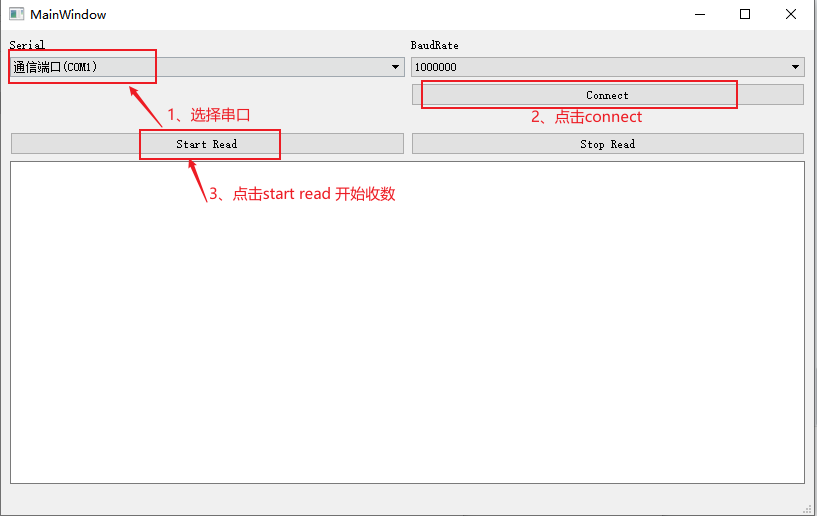
\includegraphics[scale=0.7]{firgure1.png}
\caption{打开串口接收工具}
\end{figure}

\item 重新上电BR30小板,工具显示框显示found flag, start write file表示开始收数;
\begin{figure}[H]
\centering
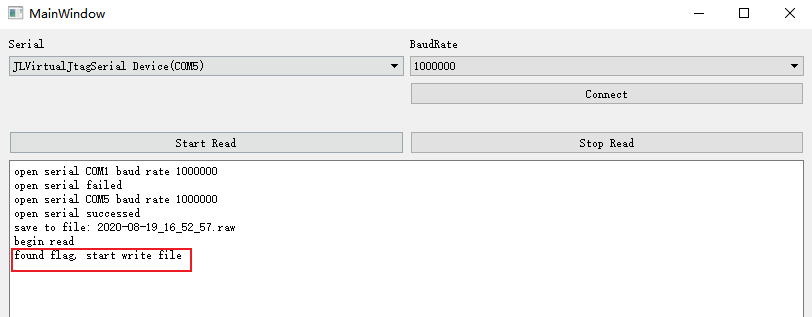
\includegraphics[scale=0.7]{firgure2.png}
\caption{开始接收数据}
\end{figure}

\item 停止收数,点击Stop Read;
\begin{figure}[H]
\centering
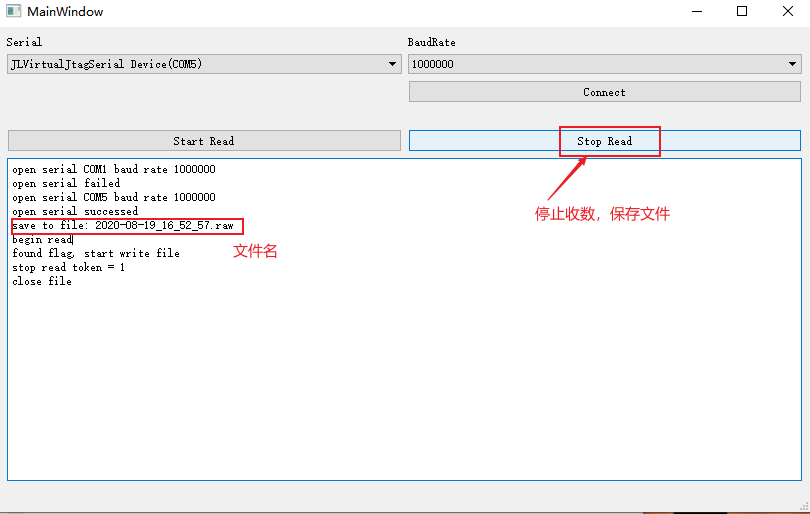
\includegraphics[scale=0.7]{firgure3.png}
\caption{停止接收数据}
\end{figure}

\item 打开保存的文件查看数据,文件开头4byte数据固定为字符串“abc”,分析数据时可不用理会,数据存储方式是X,Y或者X,Z轴数据交错存放:
\begin{figure}[H]
\centering
%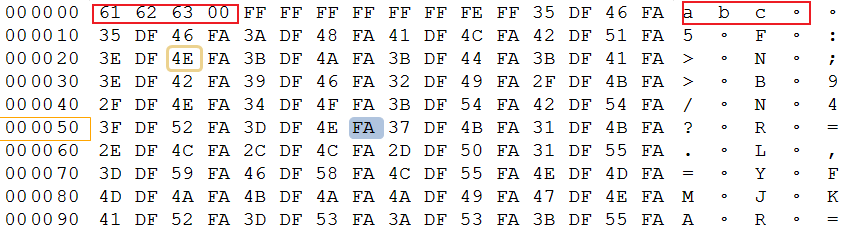
\includegraphics[height=8cm, width=16cm]{firgure4.png}
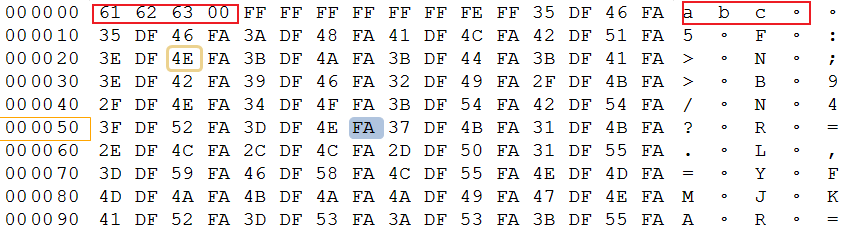
\includegraphics[scale=0.7]{firgure4.png}
\caption{检查接收数据}
\end{figure}


\end{itemize}

